%!TEX root = ../dissertation.tex
% this file is called up by thesis.tex
% content in this file will be fed into the main document

\graphicspath{{7-timbre/figures/}}

\chapter{Synthesizer-Aided Multi-Instrument Transcription}
\label{ch:timbre}

In Chapter \ref{ch:introduction}, we introduced the idea of extending a music transcription model with an additional synthesizer component that can convert the transcribed information back to the input audio, forming an analysis/synthesis framework as depicted in the encoder-decoder architecture in Figure \ref{fig:autoencoder}.
By doing so, we anticipated that the two components --- the transcriber and the synthesizer --- can work together to better translate information between the two representations, i.e. audio waveform and the transcribed semantic information of the music.
One motivation for employing such analysis/synthesis framework is that the advent of many successful deep learning techniques and the improved hardware capability may allow us to convert an audio signal completely into the constituent pieces of musical information that we want to transcribe, that are entangled in an extremely sophisticated way in the audio signal.
In the preceding chapters, we have considered deep learning solutions to various problems in music analysis and synthesis, such as monophonic pitch tracking (Chapter \ref{ch:monophonic}), music synthesis with controllable timbre (Chapter \ref{ch:synthesis}), and polyphonic music transcription (Chapter \ref{ch:adversarial}).
These problems correspond to a certain subset of the full encoder-decoder architecture, and in each chapter we discussed how the design choices in the model architecture and dataset construction affect the experimental results and the real-world applicability.

Having learned the lessons from these, in this chapter we aim to construct an automatic music transcription system that encompasses the full analysis/synthesis cycle, by considering the general problem of multi-instrument polyphonic music transcription.
We propose an autoencoder architecture that appends a synthesis model on top of a transcription model, and we verify the effects of the appended synthesizer in the experiments.
As in Chapter \ref{ch:synthesis}, the synthesizer component is capable of capturing the different aspects of various timbres in the dataset using a learned timbre space representation.
We show that the synthesizer component can serve as a regularizer to the transcriber, providing a form of prior knowledge on the spectral and temporal characteristics of the timbres. 
% \TODO{some conclusive sentence summarizing the results of this chapter}

\section{Introduction}

Multi-instrument music transcription aims to extract not only the occurrences of multiple simultaneous pitches and notes but also the types of one or more instruments corresponding to those notes.
Since it poses additional challenges to the already difficult problem of polyphonic music transcription, studies on the complete multi-instrument polyphonic transcription problem are relatively rare.
Instead, most studies on analyzing multi-instrument audio focus on either developing a discriminative model for polyphonic where timbre information is disregarded~\cite{bittner2017deepsalience} %\TODO{cite more}
or the problem of instrument recognition, while not identifying the individual notes that belongs to the recognized instruments~\cite{lostanlen2016spiral}. %\TODO{cite more}
To take both polyphonic notes and multiple instruments into account, a model has to carefully incorporate the prior knowledge of how pitch and timbre are reflected in the audio signal, e.g. using a probabilistic latent component model~\cite{benetos2015probabilistic} or a variant of non-negative matrix factorization~\cite{grindlay2009eigeninstruments}.
To produce outputs in multiple domains, these models have to include an intricate set of design choices to implement a mathematical representation of the prior knowledge.

Meanwhile, the main premise of deep learning is quite opposite of how those models are designed.
Rather than writing down the set of rules manually, layers of simple calculations can serve as a very effective function approximator, that can produce just about anything when an enough amount of data is fed to the black box.
In these models, the prior knowledge baked into the model architecture is minimal.
Take the Onsets and Frames model~\cite{hawthorne2018onsetsframes} for example; the model output has 88 dimensions corresponding to each key of the piano, but the 88 keys are treated as a separate multi-label target, without utilizing the knowledge that each key should represent a certain frequency that the quasi-periodic signal in the input follows.
Because of this lack of ``inductive bias'', deep learning models typically have to be trained with a very large amount of data; in other words, they are less sample efficient.


Generative models for transcription, such as a Bayesian network representation of spectrogram~\cite{bergkirkpatrick2014unsupervised}, takes the opposite approach.
These models define the process of generating sound entirely from the parameterized sources that typically convey a physical interpretation, such as the modeling of attack-decay-sustain-release (ADSR) curves or the energy distribution along harmonics. 
Compared to data-driven models with a lot of learnable parameters, however, those interpretable transcription models often lack the flexibility to be applicable for a wider variety of inputs.

In this chapter, we explore the possibility of finding a compromise between the two extremes.
Specifically, we examine how to induce the transcription model to make predictions such that, when synthesized back into audio, resemble the original audio input.
We do this by appending a neural music synthesis model to the transcription model, and the synthesis model is specifically designed to describe the sound generation process with a small number of interpretable parameters, which is restrictive enough to guide the transcription model to more accurate predictions, yet flexible enough to be learnable in a data-driven manner.
We evaluate this approach with a multi-instrument transcription task and show that a synthesis model can serve as an effective regularizer. % \TODO{describe qualitative improvement}

\section{Related Work}


\subsection{Multi-Instrument Music Transcription}

Transcribing polyphonic music with multiple instruments present is a particularly difficult problem and there has been relatively few successful attempts, as it requires solutions to instrument classification in addition to multiple pitch estimation.
While some approaches perform source separation and instrument recognition as a separate pre-processing step for per-instrument polyphonic transcription,~\cite{heittola2009separation,itoyama2011bayesian}, a number of approaches attempt to jointly solve the two problems, by modeling possible instruments as a constraint to non-negative matrix factorization (NMF)~\cite{grindlay2009eigeninstruments}, applying spectral templates to a probabilistic latent component model~\cite{benetos2015probabilistic}, and using a U-Net architecture to separate a multi-channel representation of audio into per-instrument transcriptions~\cite{wu2019musicnet}.
In general, joint estimation of instrument and multiple pitches allows for flexible modeling of diverse sounds and enables an end-to-end approach for multi-instrument polyphonic transcription.


\subsection{Deep Clustering}

Deep clustering~\cite{hershey2016deepclustering} is a technique for audio source separation which learns a mapping from each time-frequency bin of the input audio into an embedding space.
% During training, a pair of embedding vectors corresponding to the same source are encouraged to be closer to each other, while pushing the pairs corresponding to different sources apart from each other. To do this, 
The original formulation uses the class assignment matrix $Y = \{ y_{i,c} \}$ indicating whether element $i$ belongs to cluster $c$ and learns the embedding matrix $V = \{ \mathbf{v}_{i} \}$ as a function of the input audio that minimizes the Frobenius distance between the assignment matrix:
\begin{equation}\label{eqn:deepclustering}
\mathcal{L} = \lVert VV^\top - YY^\top \rVert_{\mathrm{F}}^2 = \sum_{i, j} \left ( \left < \mathbf{v}_i, \mathbf{v}_j \right > - \left < \mathbf{y}_i, \mathbf{y}_j \right > \right )^2.
\end{equation}
Since $\left < \mathbf{y}_i, \mathbf{y}_j \right >$ equals 1 if the elements $i$ and $j$ belongs to the same cluster and 0 otherwise, the learned embedding vectors are optimized to be as close as possible for the vectors which belong to the same cluster and as orthogonal as possible otherwise.
Alternative objective functions to Equation \ref{eqn:deepclustering} employing deep neural networks have been suggested by~\cite{wang2018deepclustering}.
The deep clustering technique has been successfully applied to the multi-speaker separation~\cite{isik2016deepclustering} and the singing voice separation problem~\cite{luo2017deepclustering}.

This chapter's work borrows the idea of deep clustering and builds an embedding space that captures the timbres of different instruments, while relying on a synthesizer component rather than inducing every pair of embedding vectors to be orthogonal to each other.
By allowing different embedding vectors to be similar but not necessarily orthogonal, the synthesizer can learn to map similar-sounding instruments to vectors that are close to each other.
Informed by this embedding space, the multi-instrument transcription model can more easily learn to classify the similar instruments than when the instruments are treated independently.


% \subsection{Source-Filter Synthesis}
% \cite{heittola2009separation} (instrument recognition)

\subsection{Generative Modeling for Transcription}

Bayesian approaches for music transcription consider the audio generation process as a probabilistic model that can describe the generated audio in terms of its sound events.
In these approaches, an audio representation such as a spectrogram is considered as an observation, and the model parameters that maximizes the observation is found using Bayesian inference techniques such as particle filtering~\cite{dubois2005harmonic}, message propagation~\cite{cemgil2006generative}, and block-coordinate ascent~\cite{bergkirkpatrick2014unsupervised}.
These models typically work well for small test datasets with a homogeneous timbral profile, but because they rely on a small, manually designed set of parameters for sound generation, they often struggle to generalize to diverse inputs.

In the spirit of utilizing the synthesizer component for transcription,
\citeA{li2017infinite} explored the idea of using on-the-fly synthesized training dataset for piano transcription, using a simple fully-connected neural network operating on the CQT representation.
\cite{choi2019drum} proposes appending a drum synthesizer component to enable fully unsupervised training of drum transcription.
The work in this chapter draws several ideas from these previous approaches of incorporating a synthesizer component into the loop, while also leveraging the flexibility and the generalizability of data-driven deep learning.

\section{Method}

We first describe the synthesizer model, followed by the modifications to the Onsets and Frames~\cite{hawthorne2018onsetsframes} transcription model made to allow the concatenation of the two models.

\subsection{Synthesizer Model}

The synthesizer model takes a per-instrument piano roll representation of symbolic music (see Figure \ref{fig:transcription-to-piano-rolls}) and uses a learned instrument embedding to predict the Mel spectrogram of the corresponding audio.
We are assuming here that predicting Mel spectrograms is equivalent to synthesizing the audio for our purposes, since we have seen in Chapter \ref{ch:synthesis} that Mel spectrograms contain most of the perceivable information present in the audio content, and the original audio can readily be reconstructed using sample-based synthesis models like WaveNet~\cite{oord2016wavenet}.

The synthesizer consists of two subcomponents, the envelope estimator and the waveshaper, respectively implementing the temporal and spectral characteristics of the sound being synthesized.
The computation in each subcomponent is performed independently for each pitch-instrument combinations, and their results are combined to obtain the resulting Mel spectrogram, as shown in Figure \ref{fig:synthesizer-architecture}.
Both components take the instrument embedding in order for the synthesized audio to exhibit different temporal and spectral behaviors depending on the instrument, and together they ensure that the synthesis model only creates harmonic sounds with the frequency corresponding to the pitch of input notes and the spectral envelope consistent among each instrument.

The envelope estimator component predicts the temporal envelope of each note, by mapping the note activities into a latent space using a one-dimensional convolution layer, followed by a FiLM layer~\cite{perez2018film} to condition on the instrument.
A GRU layer~\cite{cho2014seq2seq} is then applied in order to model the temporal behavior, such as the attack-decay-sustain-release (ADSR) curves.
Meanwhile, the waveshaper component performs a subtractive synthesis to obtain the spectrum corresponding to each pitch and instrument.
We use two types of source waves, sawtooth and triangular, to make it easily adaptable to the timbres that primarily consists of odd harmonics, such as the clarinet.
The instrument embedding is used to predict the transfer function in the Mel frequency domain to be applied to each source spectrum, which is modeled as a polynomial function mapping Mel frequencies to log magnitudes.
The Mel spectrogram corresponding to each note can then be calculated in the complex domain, by assigning a random initial phase to each pitch-instrument pair and multiplying the temporal envelope predicted by the envelope estimator.
All of the per-note Mel spectrograms are then added to obtain the final Mel spectrogram output.



\begin{figure}
	\centering
	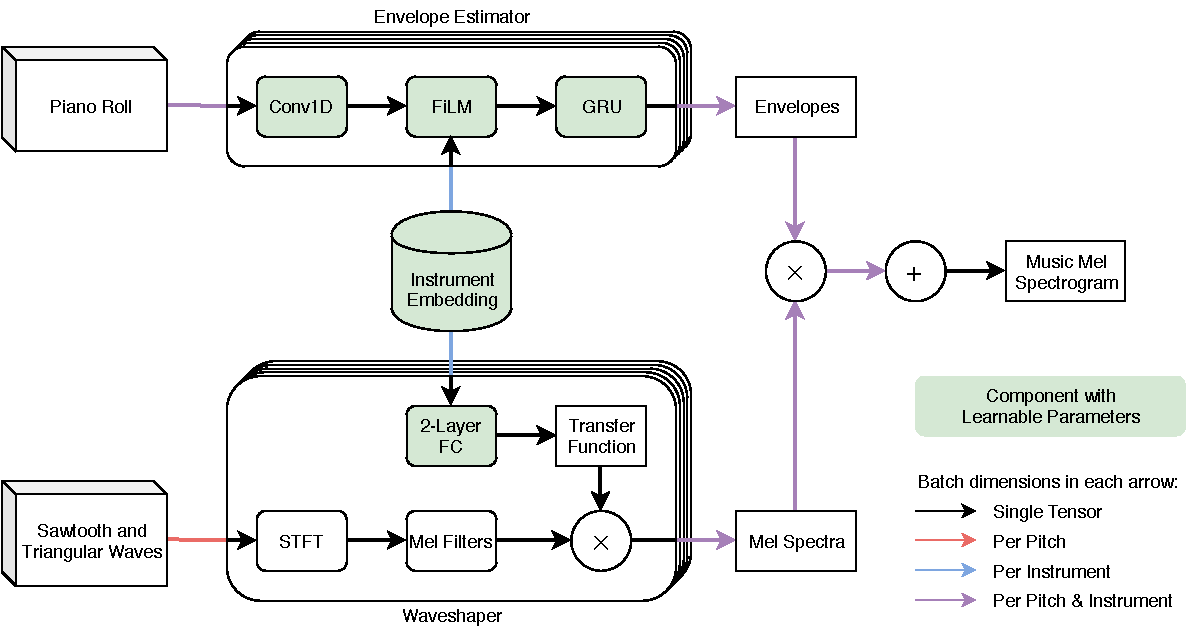
\includegraphics[width=\textwidth]{synthesizer-architecture.pdf}
	\caption{The synthesizer architecture. The temporal and spectral characteristics of each notes are respectively modeled by the envelope estimator and the waveshaper. This structure enforces each instrument to have consistent spectral and temporal envelopes across the pitch.}\label{fig:synthesizer-architecture}
\end{figure}


\subsection{Training Transcriber with Appended Synthesizer}

To append the synthesizer component to the output of the transcription model while keeping the full model differentiable, we expand the fully-connected layer predicting the frame activation to additionally predict the instrument embedding corresponding to each time-frequency bin.
Using the expanded outputs, the frame activations and the predicted embedding can be fed to the synthesizer component.
The frame activations are binarized before feeding to the synthesizer, and we use a gradient-stop for this connection.

The synthesizer model is separately trained, and the transcriber model is then optimized to minimize the sum of three losses:
\begin{equation}\label{eqn:overall-loss}
\mathcal{L}_{\text{Overall}} = \mathcal{L}_{\text{Onsets \& Frames}} + \lambda \left ( \mathcal{L}_{\text{Embedding}} + \mathcal{L}_{\text{Synthesizer}} \right )
\end{equation}
The first term, $\mathcal{L}_{\text{Onsets \& Frames}}$, is the loss of the Onsets and Frames model which is the sum of the binary cross entropy of the onsets, offsets, and frame predictions.
We define $\mathcal{L}_{\text{Embedding}}$ as the mean squared error (MSE) between the predicted instrument embedding and the ground truth, and $\mathcal{L}_{\text{Synthesizer}}$ is defined as the mean cosine distance between the predicted and the ground-truth Mel spectra:
\begin{equation}\label{eqn:cosine-distance-loss}
\mathcal{L}_{\text{Synthesizer}} = \mathbb{E}_{\hat{\mathbf{s}}, \mathbf{s}} \left [ 1 - \frac{ \hat{\mathbf{s}} \cdot \mathbf{s} }{\lVert \hat{\mathbf{s}} \rVert \lVert \mathbf{s} \rVert} \right ]
\end{equation}
where $\mathbf{s}$ follows the distribution of Mel spectra in the input audio, and $\hat{\mathbf{s}}$ is the Mel spectra predicted by the synthesizer based on the transcription predicted from $\mathbf{s}$.

\section{Experimental Setup}

We use the MusicNet dataset~\cite{thickstun2017musicnet} to train both the synthesizer and the transcriber.
The dataset contains 2,048 minutes of classical chamber music audio and labels, which comprises 330 recordings of various ensembles.
The dataset contains annotations of 11 General MIDI instruments: acoustic grand piano, harpsichord, violin, viola, cello, contrabass, french horn, oboe, bassoon, clarinet, and flute.
Different recordings in the dataset have drastically different tuning, ranging more than a semitone in some recordings which would result in a wrong transcription even by a perfect transcriber.
To alleviate this, we preprocess the dataset by running a tuning estimator implemented in librosa~\cite{mcfee2015librosa} on each track and pitch-shifted any recordings that are more than 20 cents apart from the A440 tuning.

We use the Onsets and Frames model~\cite{hawthorne2018onsetsframes} with the hidden size of 512, which contains 10 million learnable parameters.
We use a 2-dimensional instrument embedding space to represent the distribution of the 11 instruments, and the polynomial transfer functions used in the subtractive synthesis are modeled by cubic B\'{e}zier curves.
We additionally train and compare a multi-label prediction model, which replaces the last layer of the Onsets and Frames model with a multi-label binary classifier that predicts the activation of each of the 11 instruments.

The audio is resampled to 16kHz, and a training batch is composed of eight 20-second audio segments and labels.
We use Adam optimizer~\cite{kingma2015adam} with learning rate 0.0006, and the learning rate decay of factor 0.98 is applied every 1000 steps.
We ran the optimization for 180,000 steps and report the transcription accuracy evaluated on the 10 test recordings provided in the MusicNet dataset.

\section{Results}

In this section, we summarize the experimental results, first by qualitatively analyzing the behavior of the synthesizer model, followed by quantitative comparisons of transcription accuracies of the baseline and proposed transcription models.
We also introduce a web interface that allows for easier exploration of the contents of the MusicNet dataset.

\subsection{Synthesizer Output}

\begin{figure}
\centering
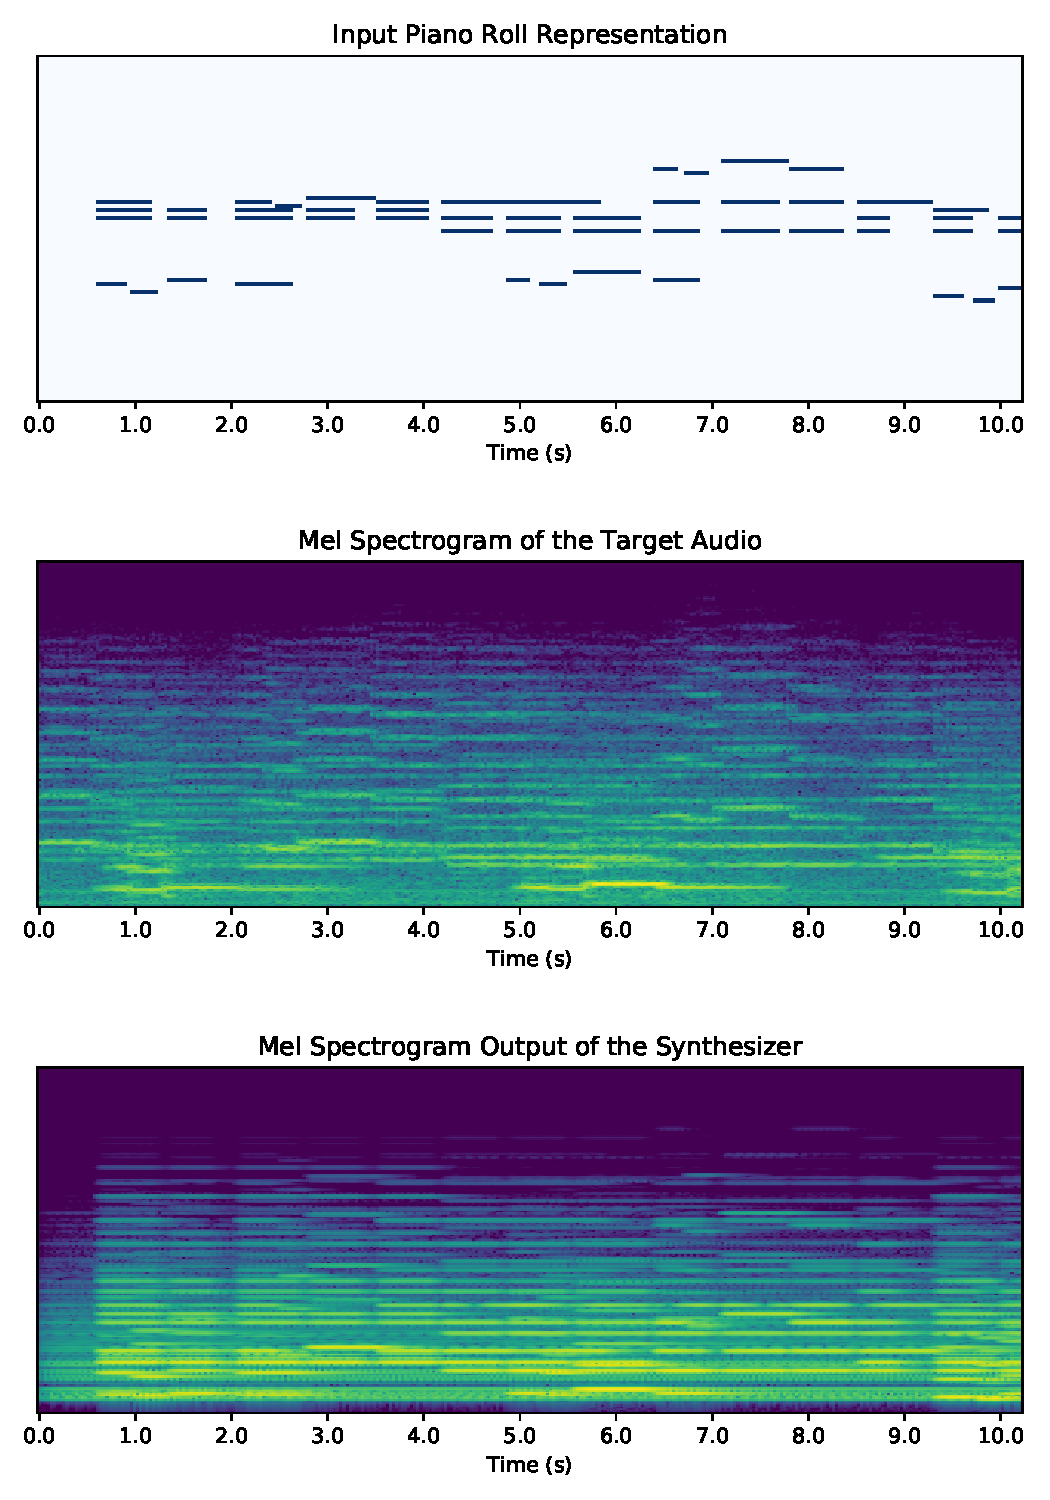
\includegraphics[width=\textwidth]{synthesizer-output.pdf}
\caption{An example of the input, target, and output representations of the synthesizer. The output resembles the target Mel spectrogram but shows a regular pattern as constrained by the synthesizer model. }\label{fig:synthesizer-output}
\end{figure}

Figure \ref{fig:synthesizer-output} shows example input, target, and output representations of the synthesizer component, and Figure \ref{fig:learned-timbre-embedding} shows the learned timbre embedding space containing the 11 instruments in the MusicNet dataset.
The input to the synthesizer contains the frame information in a piano roll format, along with the corresponding timbre embeddings (not shown in Figure~\ref{fig:synthesizer-output}).
The synthesizer is trained to predict the corresponding audio's Mel spectrogram by minimizing the cosine distance.
Figure \ref{fig:learned-timbre-embedding} indicates that the synthesizer model is able to learn a timbre embedding space that maps similar kinds of instruments into neighboring regions in the space.

Because the synthesizer is strictly limited by its architecture (Figure~\ref{fig:synthesizer-architecture}) to produce harmonic sound only, the output Mel spectrogram exhibits highly regular patterns compared to the target Mel spectrogram.
While this output Mel spectrogram may not represent an audio signal that perfectly matches the target, it motivates us to find out whether this synthesizer can give informative signals to a transcription model.

\begin{figure}
	\centering
	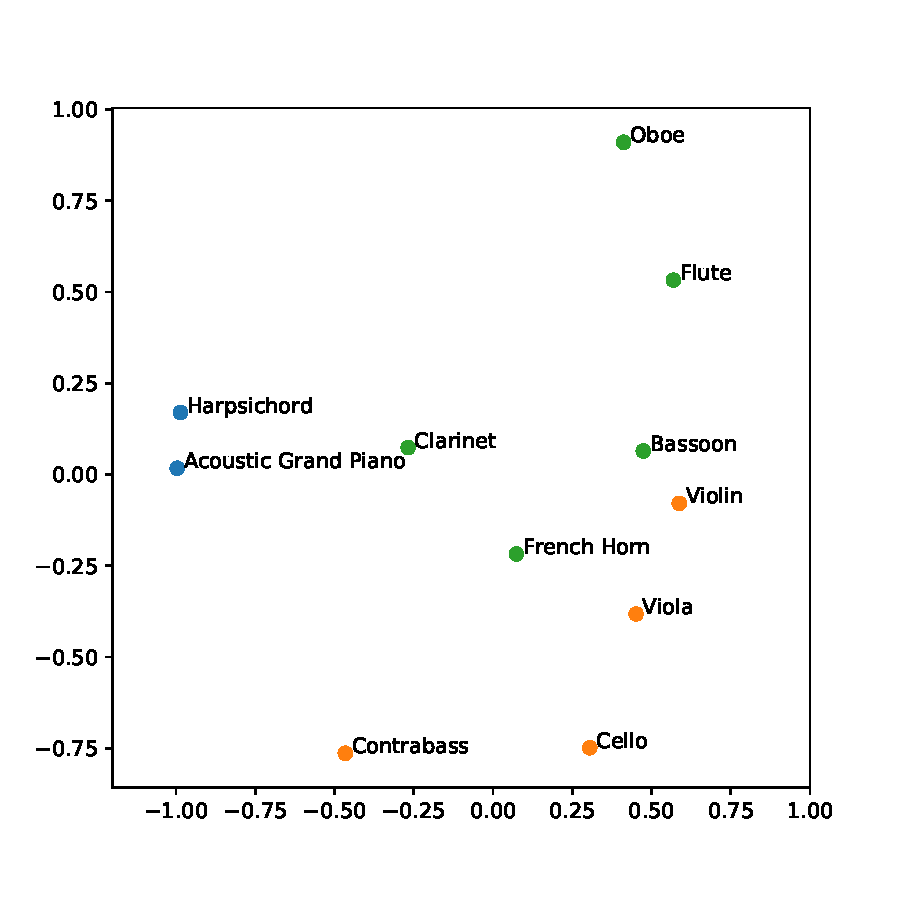
\includegraphics[width=0.75\textwidth]{cosine_distance.pdf}
	\vspace{-1em}
	\caption{The learned timbre embedding space mapping the 11 instruments in the MusicNet dataset into the corresponding points in the space. Types of instruments (keyboards, winds, and strings) are color-coded.}\label{fig:learned-timbre-embedding}
\end{figure}

\begin{table}
	\centering\small
	\begin{tabular}{l|ccc}
		& \makecell{Baseline \\ (single label)} & \makecell{Baseline \\ (multi-label)} & \makecell{Baseline \\ (synthesizer-aided)} \\ \hline
		F1 Score & 0.720 & 0.650 & \textbf{0.729} \\
		Precision & \textbf{0.736} & 0.714 & 0.735 \\
		Recall & 0.711 & 0.600 & \textbf{0.726} \\
	\end{tabular}
	\vspace{1em}
	\caption{A comparison of instrument-agnostic frame transcription accuracies for the baseline models and the proposed synthesizer-aided transcription model. The proposed model achieves better recall while staying at the same precision.}\label{tab:transcription-accuracy-comparison}
\end{table}

\subsection{Transcription Accuracy}

We compare the accuracy of the transcription model trained using the additional loss terms given by the appended synthesizer model, as in Equation~\ref{eqn:overall-loss}, with the accuracy of the equivalent transcription model trained without a synthesizer component.
Table~\ref{tab:transcription-accuracy-comparison} summarizes the frame transcription metrics of the two configuration, in addition to a multi-label prediction model that performs a multi-label classification for each instrument.
The multi-label baseline exhibits significantly lower performance in these instrument-agnostic metrics, and the proposed model slightly outperforms the single-label baseline.

\begin{figure}
	\begin{subfigure}[b]{\textwidth}
		\centering
		\parbox{0.3\textwidth}{\footnotesize\centering Ground-Truth}
		\quad
		\parbox{0.3\textwidth}{\footnotesize\centering Baseline}
		\quad
		\parbox{0.3\textwidth}{\footnotesize\centering Proposed}
		\\
		\vspace{0.5em}
		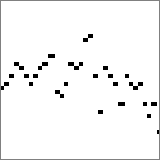
\includegraphics[width=0.3\textwidth]{cropped/2191-label.png}
		\quad
		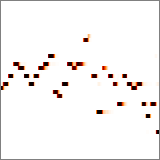
\includegraphics[width=0.3\textwidth]{cropped/2191-baseline.png}
		\quad
		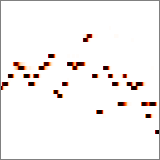
\includegraphics[width=0.3\textwidth]{cropped/2191-proposed.png}
		\caption{The proposed model correctly finds the highest note that the baseline model did not detect.}
		\label{}
	\end{subfigure}
	\begin{subfigure}[b]{\textwidth}
		\vspace{2em}
		\centering
		\parbox{0.3\textwidth}{\footnotesize\centering Ground-Truth}
		\quad
		\parbox{0.3\textwidth}{\footnotesize\centering Baseline}
		\quad
		\parbox{0.3\textwidth}{\footnotesize\centering Proposed}
		\\
		\vspace{0.5em}
		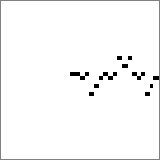
\includegraphics[width=0.3\textwidth]{cropped/2298-label.png}
		\quad
		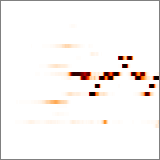
\includegraphics[width=0.3\textwidth]{cropped/2298-baseline.png}
		\quad
		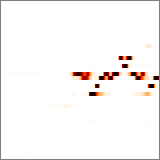
\includegraphics[width=0.3\textwidth]{cropped/2298-proposed.png}
		\caption{The proposed model makes less false positives in the silent part in the beginning of the excerpt.}
		\label{}
	\end{subfigure}
	\begin{subfigure}[b]{\textwidth}
		\vspace{2em}
		\centering
		\parbox{0.3\textwidth}{\footnotesize\centering Ground-Truth}
		\quad
		\parbox{0.3\textwidth}{\footnotesize\centering Baseline}
		\quad
		\parbox{0.3\textwidth}{\footnotesize\centering Proposed}
		\\
		\vspace{0.5em}
		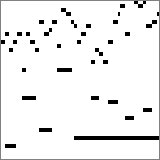
\includegraphics[width=0.3\textwidth]{cropped/2303-label.png}
		\quad
		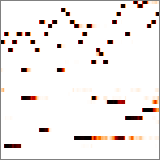
\includegraphics[width=0.3\textwidth]{cropped/2303-baseline.png}
		\quad
		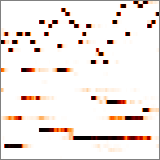
\includegraphics[width=0.3\textwidth]{cropped/2303-proposed.png}
		\caption{The proposed model better predicts the low sustained note in the latter half of the excerpt, while being more prone to false positive predictions than the baseline.}
		\label{}
	\end{subfigure}
	\caption{Examples of the frame predictions by the baseline and the proposed model, }\label{fig:frame-prediction-excerpts}
\end{figure}

Specifically, the proposed model achieves better recall than the single-label baseline while maintaining the same level of precision.
To find out how the different behaviors of the two models contribute the differences in these metrics, we visualize in Figure~\ref{fig:frame-prediction-excerpts} a few interesting excerpts that explains the better recall score of the proposed model.
Figure~\ref{fig:frame-prediction-excerpts}a is an excerpt of a solo violin track (MusicNet ID 2191) and shows that the proposed model is able to identify the highest note in the input that is not detected by the baseline model.
In Figure~\ref{fig:frame-prediction-excerpts}b, which is the beginning of a solo cello piece (MusicNet ID 2298), the baseline model produces frame activations of a few notes before the first note, falsely predicted from the background noise in the input audio.
Although the transcription metrics are not affected in this case since the activation values are below the threshold, it shows that the synthesizer model can suppress false predictions by the transcription model to a certain degree.
Finally, in a solo piano excerpt shown in Figure~\ref{fig:frame-prediction-excerpts}c, the low sustained note in the latter half of the input is better predicted by the proposed model than the baseline.
Transcription of a long sustained piano note is difficult because of the volume decay of a note, and this example implies that the appended synthesizer is able to encourage an accurate prediction of long notes.
In all of these cases, the synthesizer helps in more accurately detecting frames, which in turn contributes to the better transcription metrics.


\begin{table}[b!]
	\centering\small
	\begin{tabular}{l|ccc|ccc}
		& \multicolumn{3}{c|}{\makecell{Baseline \\ (multi-label)}}
		%& \quad\quad
		& \multicolumn{3}{c}{\makecell{Proposed \\ (synthesizer-aided)}} \\
		& F1 & Precision & Recall & F1 & Precision & Recall \\ \hline
		Acoustic Grand Piano & 0.667 & 0.694 & 0.650 & 0.546 & 0.739 & 0.435 \\
		Violin & 0.467 & 0.433 & 0.590 & 0.213 & 0.610 & 0.136 \\
		Viola & 0.195 & 0.128 & 0.412 & 0.233 & 0.290 & 0.209 \\
		Cello & 0.402 & 0.364 & 0.575 & 0.331 & 0.717 & 0.252 \\
		French Horn & 0.255 & 0.164 & 0.602 & 0.246 & 0.218 & 0.299 \\
		Bassoon & 0.290 & 0.213 & 0.473 & 0.065 & 0.152 & 0.043 \\
		Clarinet & 0.386 & 0.305 & 0.526 & 0.376 & 0.332 & 0.440 \\
	\end{tabular}
	\vspace{1em}
	\caption{Per-instrument accuracy of the multi-instrument baseline and the proposed model, showing only the instruments in the test tracks. The multi-instrument baseline generally outperforms the proposed model, which although shows higher precision across all instruments.}\label{tab:multilabel-performance-comparison}
\end{table}

\subsection{Multi-Instrument Transcription}

In this subsection, we compare the multi-instrument transcription performance of the proposed model with the multi-label baseline model.
The instrument labels are assigned by finding the nearest instrument embedding to the embedding vector predicted by the transcription model.
Table~\ref{tab:multilabel-performance-comparison} summarizes the transcription metrics for each instrument and indicates that the proposed model actually performs worse than the multi-label baseline, despite the advantages in the instrument-agnostic evaluation in the previous subsection.
One contributing factor for the lower performance is that the nearest-neighbor assignment of instrument labels cannot produce the same pitch activated by multiple instruments, i.e. playing in unison.
While the improvement in the individual multi-instrument performance remains a future work, the visualization of  Figure~\ref{fig:multi-instrument-example} shows that the model is capable of classifying the different classes of instruments, such as the piano and the strings.



\begin{figure}
	\centering
	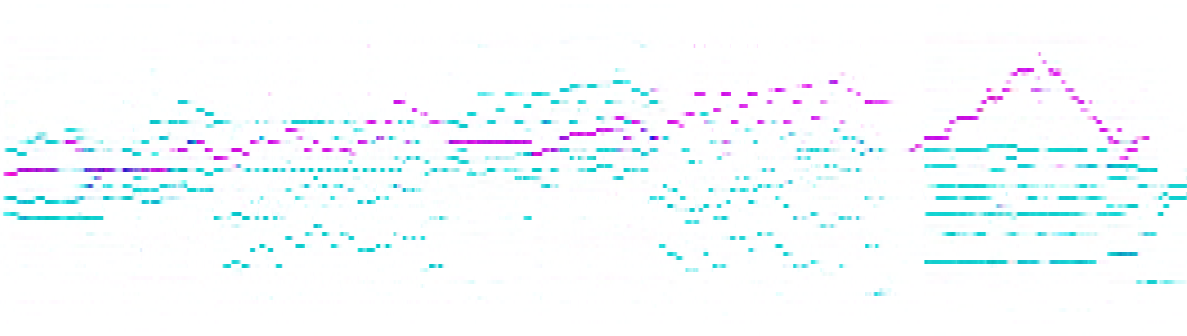
\includegraphics[width=\textwidth]{2628.png}
	\caption{An example of multi-instrument transcription of a violin piece accompanied by piano (MusicNet track 2628), where the predictions of keyboard and string instruments are color-coded in cyan and magenta, respectively. }\label{fig:multi-instrument-example}
\end{figure}

\subsection{MusicNet Inspector}

\begin{figure}[t]
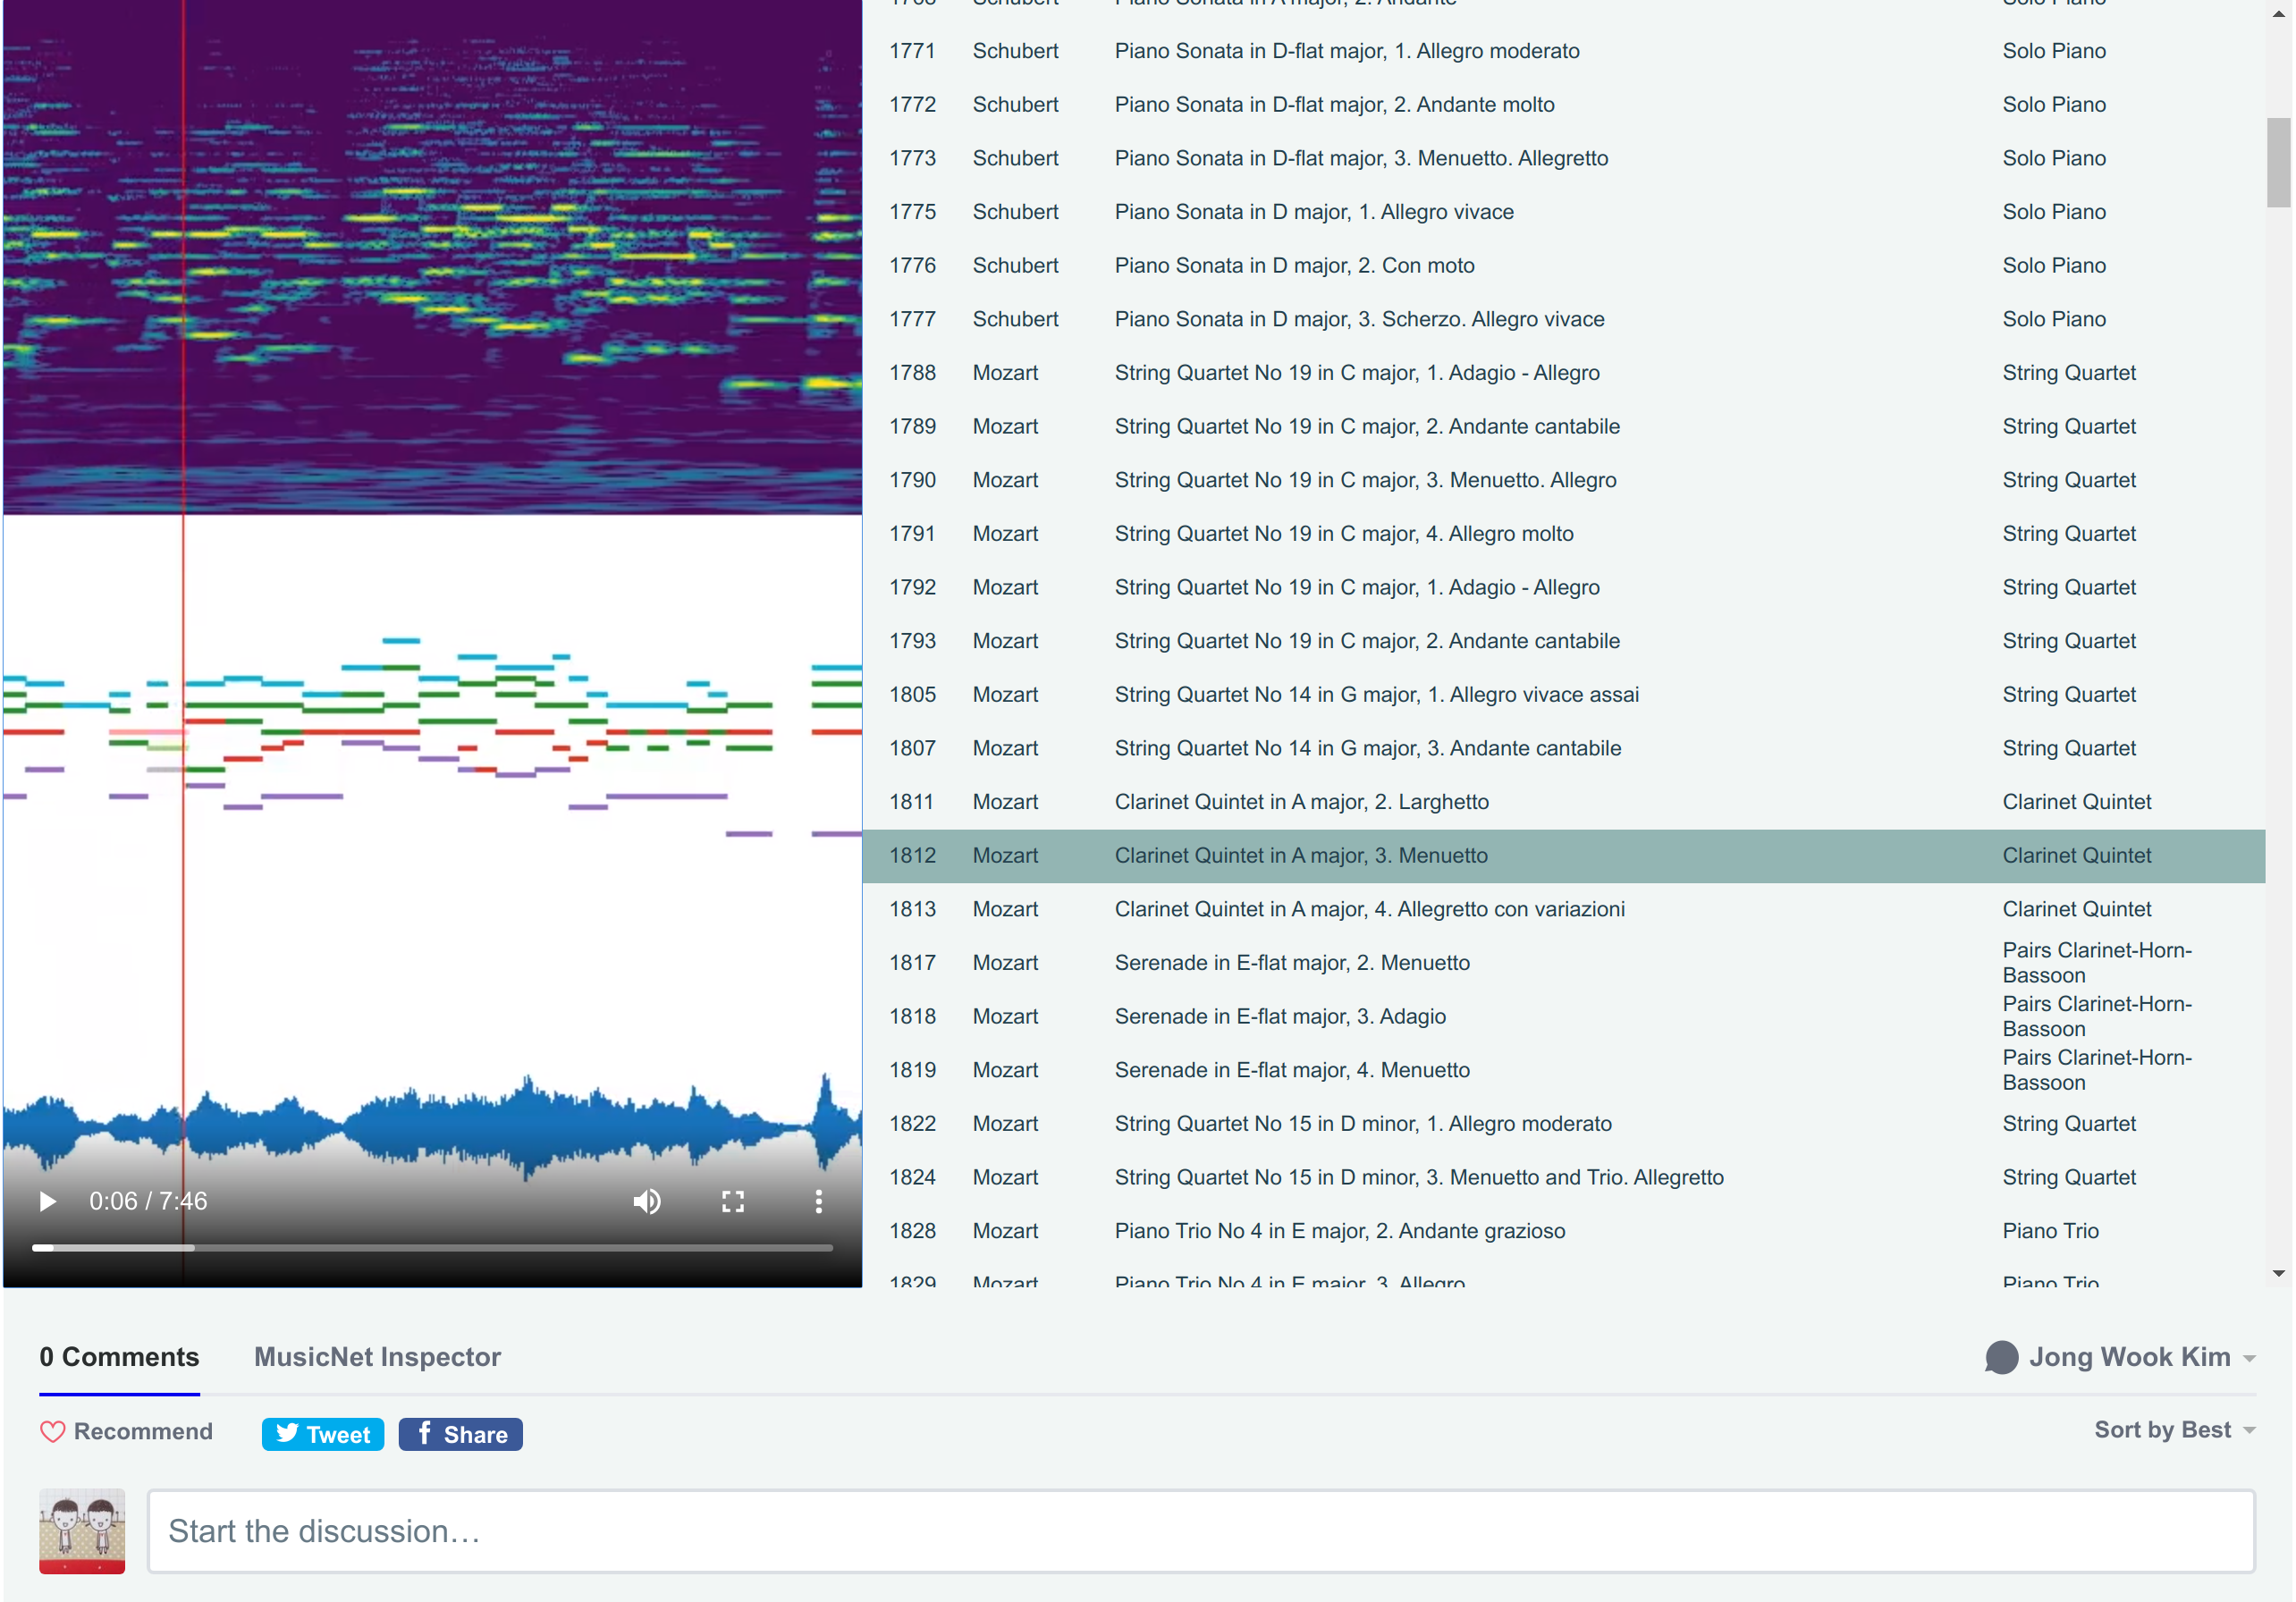
\includegraphics[width=\textwidth]{inspector.png}
\caption{The MusicNet Inspector web interface. Users can select among the 330 tracks in the MusicNet dataset, and the selected track is played together with the CQT, piano roll, and amplitude visualizations.}\label{fig:musicnet-inspector}
\end{figure}

Finally, we introduce a web interface\footnote{\url{https://musicnet-instpector.github.io}} developed for easy inspection of the audio tracks in the MusicNet dataset, which helped identify the characteristics and imperfections of the music and the annotations in the dataset.
The UI is shown in Figure~\ref{fig:musicnet-inspector}; the users can select one of the 330 tracks in the list showing the details of each track, and a video containing a CQT representation, color-coded piano-roll representation, and an audio amplitude visualization is played together with the audio.
Additionally, the users can participate in the discussion about each track, e.g. any errors in the annotations, in the comment section.
This interface can serve as a useful tool for researchers using the MusicNet dataset, providing an easy way to inspect the content of the dataset.

\section{Future Work}

The experimental results presented above has shown that a marginal improvement by the appended synthesizer component is possible. However, significant further work is required to prove the practical viability of the idea.
First of all, although MusicNet is the largest freely available dataset for multiple-instrument music transcription, it contains a non-negligible amount of inaccuracy in the annotations.
This is largely because the annotations were obtained by matching each audio track with a MIDI file containing the same piece using dynamic time warping~\cite{thickstun2017musicnet}.
This caused many inaccurate time mappings near the beginning and the end of each track, and there exist a few cases where inaccurate annotations continue over extended periods, because the music content of the audio and the MIDI file sometimes do not exactly match due to different repetitions or revisions of the music.
Furthermore, because of the inhomogeneous sources of the audio tracks, the recording conditions and the tuning vary significantly, which made the model training even more difficult, given the relatively small number of tracks in the dataset.
While the availability of a significantly larger and more accurate dataset is desirable, some of the drawbacks can be alleviated by performing data augmentation~\cite{mcfee2015muda} such as pitch shifting.
Since the audio input is not volume-normalized during training, improved robustness to different dynamic ranges of audio can be achievable by augmenting the training data with the variations in the audio volume.

We have used the cosine distance loss (Equation~\ref{eqn:cosine-distance-loss}) which is invariant to the scaling of either the predicted or the target Mel spectrograms, because the annotations does not contain the velocity information.
If a dataset containing the velocity information can be obtained, alternative loss functions such as spectral convergence~\cite{sturm2013classification} can be used for more accurate prediction of Mel spectrograms by the synthesizer.

% using onset info, dot product space, Lipschitz

\section{Conclusions}

In this chapter, we have explored the overarching idea of this thesis: using a music synthesis model to achieve better music transcription performance.
To do so, we have proposed a novel synthesizer architecture which is expressive enough to learn the distribution of different instruments, while being restricted to produce only harmonic sounds matching the input and also having a low number of parameters to be able to effectively serve as a regularizer to a transcription model.
We observed improved performance when the transcription model is appended by a pre-trained music synthesis model, which can help the transcriber achieve better recall while suppressing incorrect predictions.
Additionally, we have tested the multi-instrument transcription performance of the same setup and introduced a web interface for easier navigation of the MusicNet dataset used in the experiments.

This chapter concludes the technical work of this thesis, which started with proposing a framework for deep learning-based music analysis tasks (Chapter~\ref{ch:monophonic}), followed by introducing a WaveNet-based music synthesis model that can also learn the distribution of instrumental timbre (Chapter~\ref{ch:synthesis}) and an adversarial technique that can impose a music language model on an existing transcription model (Chatper~\ref{ch:adversarial}).
We continue our discussion of our findings so far in the context of the series of research questions raised in Chapter~\ref{ch:introduction}, as well as about the implications and the prospects of this line of research, in the next and final chapter of this thesis.


